\documentclass[UTF8]{ctexart}
\usepackage{amsmath}
\usepackage{graphicx}
\usepackage{float}
\usepackage{subfigure}
\usepackage{amsthm}
\usepackage{listings}
\usepackage{xcolor}
\lstset{
    basicstyle=\tt,
    %行号
    numbers=left,
    rulesepcolor=\color{red!20!green!20!blue!20},
    escapeinside=``,
    xleftmargin=2em,xrightmargin=2em, aboveskip=1em,
    %背景框
    framexleftmargin=1.5mm,
    frame=shadowbox,
    %背景色
    backgroundcolor=\color[RGB]{245,245,244},
    %样式
    keywordstyle=\color{blue}\bfseries,
    identifierstyle=\bf,
    numberstyle=\color[RGB]{0,192,192},
    commentstyle=\it\color[RGB]{96,96,96},
    stringstyle=\rmfamily\slshape\color[RGB]{128,0,0},
    %显示空格
    showstringspaces=false
}


\title{}
\author{李子龙\\201818000807036}


\begin{document}
\tableofcontents
\maketitle
\section{有阻尼情况下的受驱单摆}
\subsection{极限情况的分析}
运动方程是:
\begin{equation}
\label{1}
\frac{d^2\theta}{dt^2}=-mgsin\theta-\kappa l\frac{d\theta}{dt}+f_0cosw_0t,
\end{equation}
\qquad对以上方程进行无量纲化,作变换:$t_1=\sqrt{\frac{l}{g}}t$,$w_0=\sqrt{\frac{g}{l}}w_0$。从而新方程为(在新方程中,仍用$t$来标记$t_1$):
\begin{equation}
\label{2}
\frac{d^2\theta}{dt^2}+K\frac{d\theta}{dt}+sin\theta=Fcosw_0t,
\end{equation}
\qquad考虑一个可以研究的极限情况,$F\ll1,\theta\ll1$。此时方程可以近似为:
\begin{equation}
\label{3}
\frac{d^2\theta}{dt^2}+K\frac{d\theta}{dt}+\theta=Fcosw_0t,
\end{equation}
\qquad考虑到$K>0$,等式右端为0时的齐次方程的通解为:$Ae^{\lambda_1t}+Be^{\lambda_2t}$,$\lambda_1,\lambda_2=\frac{-K\pm\sqrt{a^2-4}}{2}$。$\lambda_1,\lambda_2$的实部都是负的,因而以上两项都是指数衰减的函数,在$t\rightarrow\infty$时,迅速趋向于0。
对于公式\ref{3}的特解,可以考虑如$C_1cosw_0t+C_2sinw_0t$的形式,可以解得:$C_1=\frac{F(1-w^2)}{K^2w^2+(1-w^2)^2},C_2=\frac{KFw}{K^2w^2+(1-w^2)^2}$,从而特解为:$\frac{F}{\sqrt{K^2w^2+(1-w^2)^2}}cos(w_0t+\phi_0)$。所以,在$t$很大时,单摆表现出三角函数的运动周期,同时,振幅由上式给出。\par
以上的分析描述了单摆运动的很多情形。比如,在$F=0.2,w_0=4,K=0.2$时,由以上分析给出的振幅为0.0132,这与模拟的结果非常一致。
\begin{figure}[H]
	\centering
	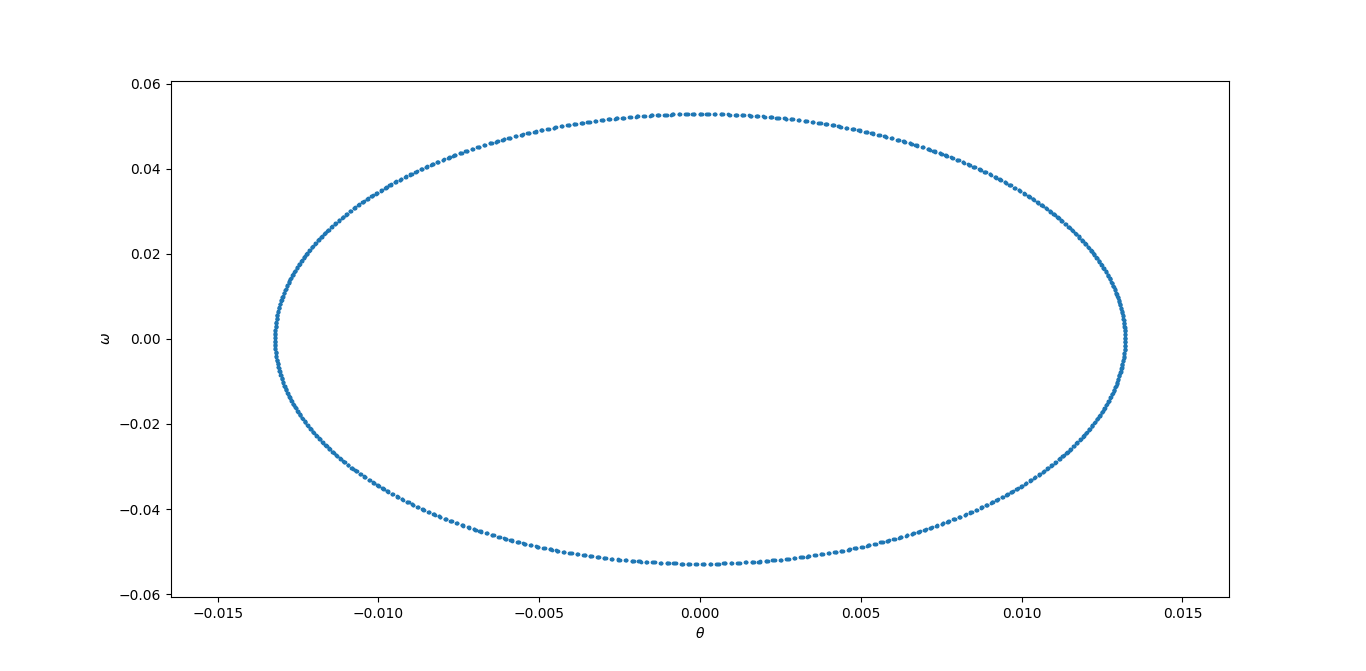
\includegraphics[width=0.7\linewidth]{F.png}
	\caption{$F=0.2,w_0=4$}
\end{figure}
更一般的观察发现,以上分析对$F$不是很小的某些情形也成立,这取决于$F/w_0^2$的大小,比如$F=6,w_0=4,K=0.2$时与分析的结果符合仍然很好。
\begin{figure}[H]
	\centering
	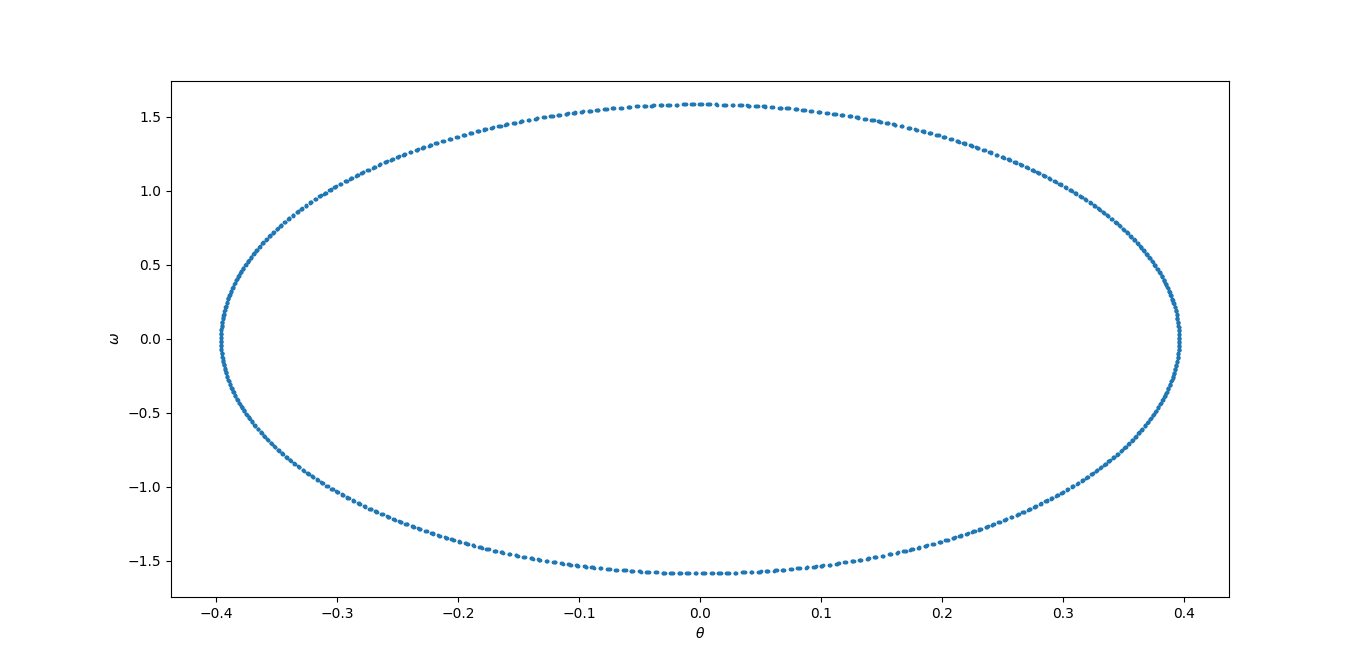
\includegraphics[width=0.7\linewidth]{F_1.png}
	\caption{$F=6,w_0=4$}
\end{figure}
\subsection{python具体实现}
equ.\ref{2}可以写成两个一阶的微分方程:
\begin{equation}
\left\{
\begin{array}{lr}
\frac{dy}{dt}=-KY-\theta+Fcosw_0t,& \\
\frac{d\theta}{dt}=y,
\end{array}
\right.
\end{equation}
\qquad首先定义了一个自己的ODE函数,它需要变量的导数方程、初始条件以及所求时间点为参数,在具体实现中采用了龙格库塔法,因为直接的欧拉法收敛的效果并不好。
\begin{lstlisting}[language=Python]
def my_ode(func,begin_value,time_list):
\end{lstlisting}
\qquad然后定义了一个专门求解有阻尼受迫振动单摆的对象。
\begin{lstlisting}[language=Python]
class pelunum_resist_drive(object):
\end{lstlisting}
\qquad对象的Pelunum函数调用ODE函数对设定的参数进行模拟,返回的是$\theta(t)$和$y(t)$。
\begin{lstlisting}[language=Python]
def Pelunum(self):
\end{lstlisting}
\begin{figure}[H]
	\centering
	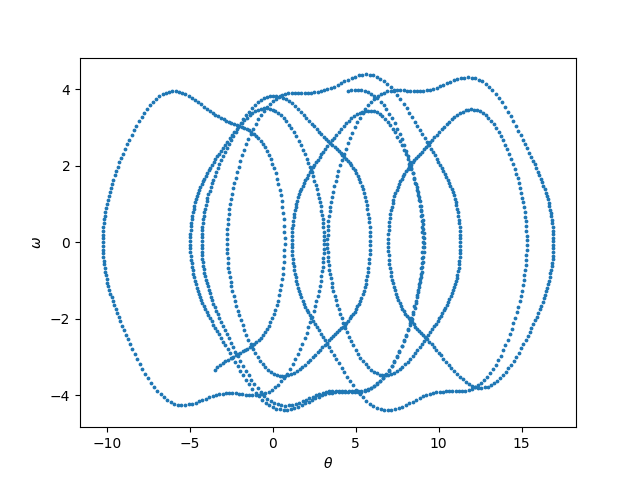
\includegraphics[width=0.7\linewidth]{mess.png}
	\caption{一个混沌解$F=3.2,w_0=2/3,K=0.5$。}
\end{figure}
\section{二阶龙格库塔法的证明}
\begin{equation}
y(t+\tau)=y(t)+y'(t)\tau+\frac{y''(t)}{2}\tau^2+O(\tau^3),
\label{4}
\end{equation}
\qquad设,$y(t+\tau)$可以表达成以下的形式:
\begin{equation}
y(t+\tau)=y(t)+c_1\alpha_1+c_2\alpha_2,
\label{5}
\end{equation}
\qquad其中:
\begin{equation}
\left\{
\begin{array}{lr} % \begin{eqnarray}好像也可以。
\alpha_1=\tau g(y,t), &\\
\alpha_2=\tau g(y+v_{21}\alpha_1\tau,t+v_{21}\tau).
\end{array}
\right.
\end{equation}
\qquad比较equ.\ref{4}和equ.\ref{5},可以得到:$\alpha_1+\alpha_2=1,\alpha_2v_{21}=\frac{1}{2}$,在此限制下可以取:$\alpha_1=\alpha_2=\frac{1}{2},v_{21}=1$。
\par证毕。\qedsymbol 
\end{document}
